\section{Hadronic observables and limits on joint recovery}
\label{sec:part-higher-dimensional}
\label{sec:part-q3}

The unfoldings that add $E_{\mathrm{avail}}$, $q_3$, and $W$ preserve the normalization and agree with the lower-dimensional results in the tested projections (Sec.~\ref{sec:higher-dimensional-extension}). Recovery of the joint distribution and uncertainty coverage at the reported resolution remain unestablished. The closure and prior-dependence studies show where recovery fails (Secs.~\ref{sec:higher-dimensional-closure} and~\ref{sec:higher-dimensional-prior}). The study in Sec.~\ref{sec:fived16-prr} probes why the estimator retains part of the prior at two simulated truths.

\subsection{Extension to \texorpdfstring{$E_{\mathrm{avail}}$, $q_3$, and $W$}{available energy, momentum transfer, and hadronic mass}}
\label{sec:higher-dimensional-extension}
\label{sec:3d}
\label{sec:uq-higherdim}

Adding available hadronic energy and three-momentum transfer to the muon momenta gives the three- and four-dimensional (3D and 4D) central values. Both use the \estMultiD{} in Table~\ref{tab:estimators-matrix} and have no reported covariance. With hadronic invariant mass added, the same estimator gives the \resSixteen{}. The \resFiveAxis{} uses the \estPurity{}.

\label{sec:3d-spectrum}
The 3D available-energy spectrum peaks at low recoil. It falls monotonically from $2.18\times10^{-38}\,\mathrm{cm}^2/(\mathrm{GeV}\,\text{nucleon})$ in the lowest bin to $6.7\times10^{-41}\,\mathrm{cm}^2/(\mathrm{GeV}\,\text{nucleon})$ in the wide $[3,100]~\mathrm{GeV}$ bin, with most of the cross section below about $0.8~\mathrm{GeV}$.
\label{sec:3d-anchor}Summing over $E_{\mathrm{avail}}$ gives an integral of about $3.07\times10^{-38}\,\mathrm{cm}^2$ per nucleon, within $0.141\%$ of the 2D result over the 205 reported muon bins. The ratios of individual muon bins have a standard deviation of about $3.7\%$.

\label{sec:3d-2p2h}
Below $E_{\mathrm{avail}}=0.4~\mathrm{GeV}$, the 3D projection exceeds the GENIE 2.12.10 central prediction by $8\%$ to $36\%$, an excess the tested model variations do not fully explain. Adding the Valencia meson-exchange current (MEC) contribution, which supplies two-particle--two-hole (2p2h) strength, raises the prediction in all three low-energy bins and closes $52\%$ of the integrated gap below $0.4~\mathrm{GeV}$ (Fig.~\ref{fig:modedecomp}). The largest remaining shortfall is in $0.10\leq E_{\mathrm{avail}}<0.20~\mathrm{GeV}$. The tested variations in pion final-state interactions shift this part of the spectrum by less than $1\%$.

\begin{figure}[tbp]
  \centering
  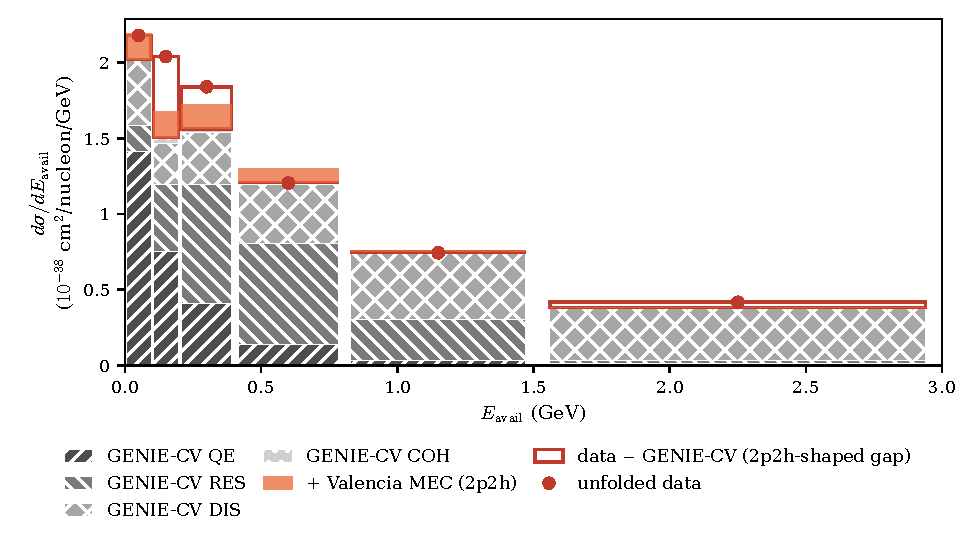
\includegraphics[width=\textwidth]{figures/mode_decomp_mec_eavail_central.pdf}
  \caption{Adding the Valencia 2p2h contribution to GENIE 2.12.10 closes $52\%$ of the integrated gap between the 3D available-energy projection and the central prediction below $E_{\mathrm{avail}}=0.4~\mathrm{GeV}$. The stacked gray histograms show quasielastic, resonant, coherent, and deep-inelastic contributions to the central prediction. The orange histogram adds the Valencia meson-exchange current (MEC) contribution, which supplies two-particle--two-hole (2p2h) strength. The outline marks the difference between data and the central prediction before adding 2p2h.}
  \label{fig:modedecomp}
\end{figure}

\label{sec:4d}
The joint $E_{\mathrm{avail}}$--$q_3$ projection reveals variation in momentum transfer at fixed visible energy. Reconstructed $q_3$ combines the muon kinematics with a distinct calorimetric recoil estimate (Sec.~\ref{sec:observable-definitions}). In the 4D purity-baseline check, the lowest $E_{\mathrm{avail}}$ bin is 1.21 times the MINERvA Tune v1 prior after integrating over $q_3$. The ratio approaches unity in the transition between quasielastic and $\Delta$-resonance production and rises to 1.16--1.23 at high $E_{\mathrm{avail}}$. The joint projection shows ratios as low as 0.66 at intermediate $E_{\mathrm{avail}}$ and low $q_3$, rising toward larger $q_3$ in the same available-energy range (Fig.~\ref{fig:q3excess}).

\begin{figure}[tbp]
  \centering
  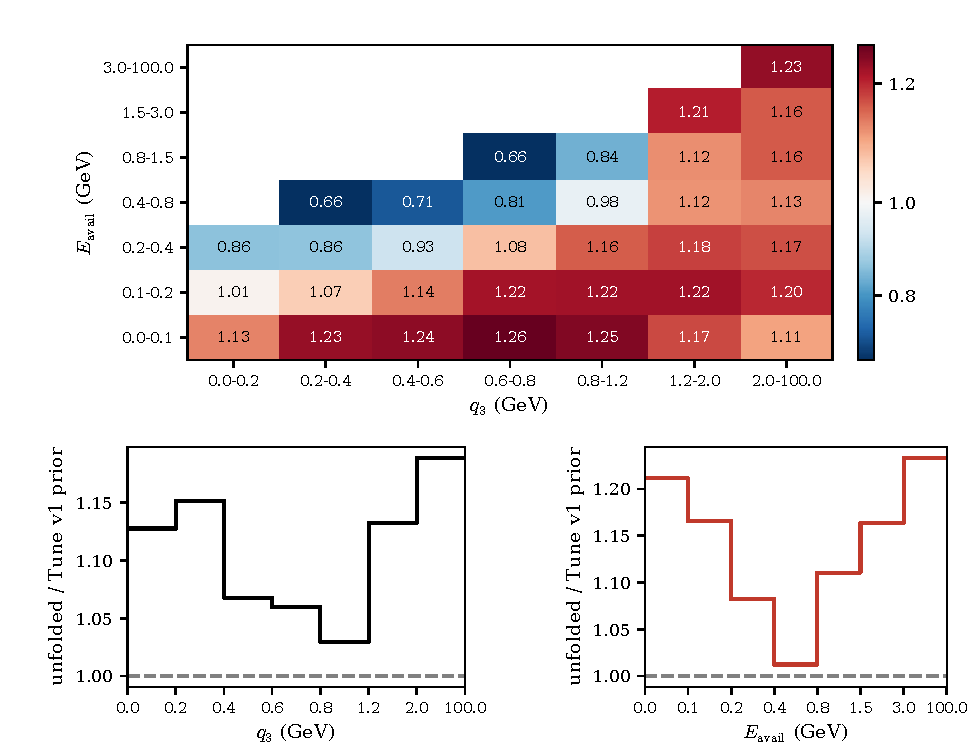
\includegraphics[width=\textwidth]{figures/q3_excess_projection.pdf}
  \caption{At intermediate $E_{\mathrm{avail}}$, the ratio of the 4D purity-baseline unfolding to the MINERvA Tune v1 prior falls to 0.66 at low $q_3$ and rises toward larger $q_3$. The upper panel shows the joint $E_{\mathrm{avail}}$--$q_3$ projection, with kinematically empty cells left blank. The lower panels show the $q_3$ and $E_{\mathrm{avail}}$ marginals.}
  \label{fig:q3excess}
\end{figure}

On the grid shared with the published MINERvA low-recoil measurement~\cite{MINERvA:2022incl}, the refined 4D central values are $9.2\%$ and $6.0\%$ above the published values in the $q_3$ intervals $[0.4,0.6)$ and $[0.6,1.2)~\mathrm{GeV}/c$, respectively, for $E_{\mathrm{avail}}<0.4~\mathrm{GeV}$ and $p_\parallel<20~\mathrm{GeV}/c$.

\label{sec:eavailw}

Adding $W$ changes the normalization and the single-axis projections only slightly. The \resFiveAxis{} integral is 1.0011 times that of the corresponding 4D purity unfolding. The median differences in the one-dimensional projections on the four shared axes range from $0.3\%$ to $1.5\%$. The $W$ projection is finite and nonnegative in all six bins. The existing 4D inputs determine reconstructed $W$ (Sec.~\ref{sec:observable-definitions}). Resolving true $W$ therefore relies on the simulated relationship between those inputs and the joint truth.

\label{sec:eavailw-map}
In the \resFiveAxis{}, the low-recoil excess over Tune v1 is concentrated at \mbox{$W<1.1~\mathrm{GeV}$} (Fig.~\ref{fig:available-energy-hadronic-mass}). Below $E_{\mathrm{avail}}=0.4~\mathrm{GeV}$ the ratios there range from 1.23 to 1.26. The unfolded yield falls below the prior at $0.2\leq E_{\mathrm{avail}}<0.8~\mathrm{GeV}$ and $1.4\leq W<1.8~\mathrm{GeV}$. For $1.5\leq E_{\mathrm{avail}}<3~\mathrm{GeV}$, the largest ratio is 1.30 at \mbox{$W<1.1~\mathrm{GeV}$}, whereas the largest cell-integrated excess is $4.1\times10^{-40}\,\mathrm{cm}^2$ per nucleon at $1.8\leq W<2.2~\mathrm{GeV}$.

\begin{figure}[tbp]
  \centering
  % The source file stacks the panels. Display its upper and lower halves side by side to preserve the left/right references in the caption.
  \sbox{0}{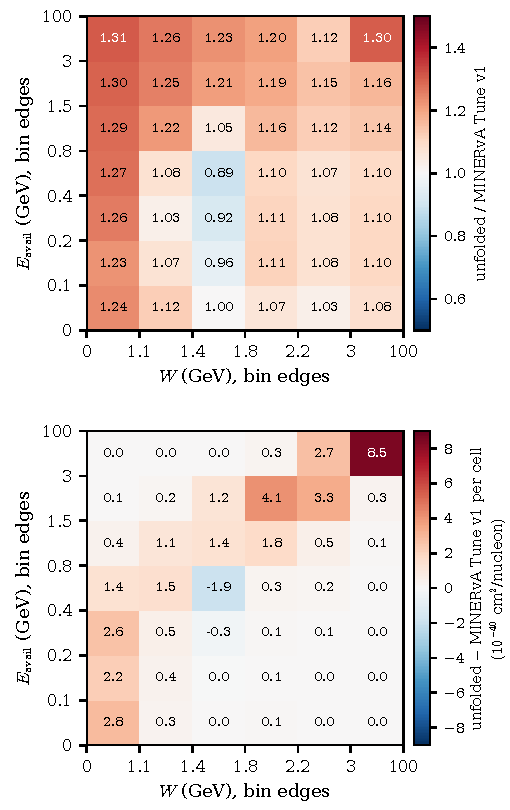
\includegraphics{figures/paper_fig2_joint.pdf}}%
  \edef\showJointPanels{%
    \noexpand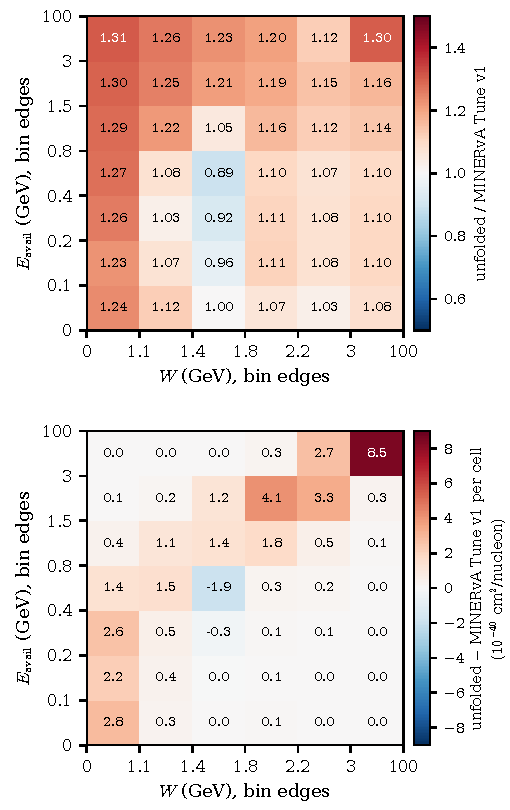
\includegraphics[trim=0 \the\dimexpr\ht0/2\relax\space 0 0,clip,width=0.46\noexpand\linewidth]{figures/paper_fig2_joint.pdf}%
    \noexpand\hfill
    \noexpand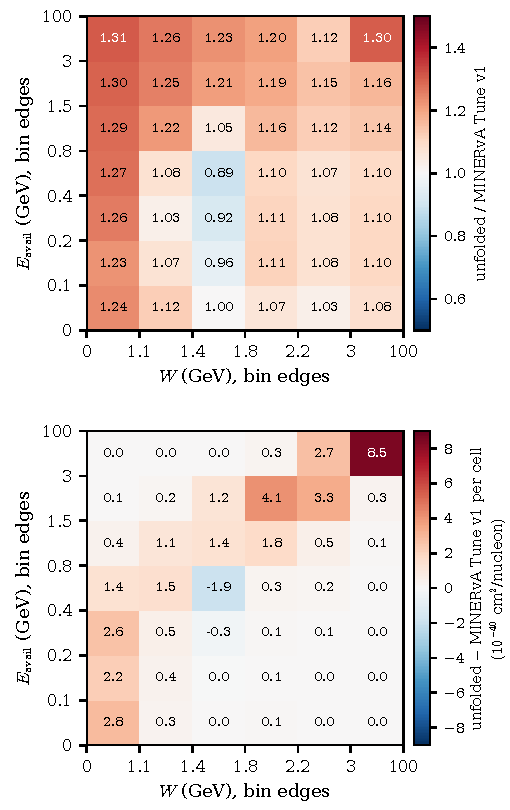
\includegraphics[trim=0 0 0 \the\dimexpr\ht0/2\relax,clip,width=0.46\noexpand\linewidth]{figures/paper_fig2_joint.pdf}%
  }%
  \showJointPanels
  \caption{The low-recoil excess of the \resFiveAxis{} over the MINERvA Tune v1 prior is concentrated at $W<1.1~\mathrm{GeV}$. The upper panel gives the ratio and the lower panel the difference of the cell-integrated cross sections in units of $10^{-40}\,\mathrm{cm}^2$ per nucleon, projected onto $(E_{\mathrm{avail}},W)$. The cells are drawn with equal size and labeled by their physical bin edges. The last interval on each axis spans $[3,100]~\mathrm{GeV}$. The comparison uses central values only.}
  \label{fig:available-energy-hadronic-mass}
  \label{fig:eavailWexcess}
\end{figure}

\subsection{Five-dimensional estimators and reporting regions}
\label{sec:five-dimensional-reporting}

The \resFiveAxis{} supplies the fine-grid distribution in Fig.~\ref{fig:available-energy-hadronic-mass} and the diagnostic covariance $C_Z$. It uses the \estPurity{}, which assigns binned purity weights before unbinned training. The \resSixteen{} uses the refined negative-weight subtraction of Sec.~\ref{sec:omnifold-implementation}.

The sixteen cells are rectangular regions in $(p_T,p_\parallel,E_{\mathrm{avail}},q_3,W)$. We first divide the muon plane at $p_T=\fvval{h2-mid-pt}~\mathrm{GeV}/c$ and $p_\parallel=\fvval{h2-mid-pz}~\mathrm{GeV}/c$ within the reported ranges $[0,4.5]$ and $[1.5,60]~\mathrm{GeV}/c$, respectively. Within each muon quadrant, the hadronic subdivisions have edges $(\fvval{h2-edges-eavail})~\mathrm{GeV}$ in $E_{\mathrm{avail}}$, $(\fvval{h2-edges-q3})~\mathrm{GeV}/c$ in $q_3$, and $(\fvval{h2-edges-W})~\mathrm{GeV}$ in $W$. The sixteen reporting-region IDs, R00--R15, identify the retained regions in Table~\ref{tab:five-dimensional-regions}. They were formed by merging supported boxes of this coarse grid using reconstructed purity. The coarse grid has \fvval{h2-nsupported} supported boxes, each with an expected reconstructed signal yield and selected truth weight of at least 1000 at the data exposure. We report the integrated cross section per nucleon in each region.

\begin{table}[tbp]
  \centering
  \caption{Definitions of the sixteen reporting regions. The $p_T$, $p_\parallel$, and $q_3$ intervals are in $\mathrm{GeV}/c$, and the $E_{\mathrm{avail}}$ and $W$ intervals are in $\mathrm{GeV}$. The rows are grouped by muon quadrant. Four cells (\fvval{h2-lowstab-cells}) have a low fraction of selected truth events reconstructed in the same cell. The first three select high available energy, low momentum transfer, and low mass. R15 spans the full mass interval.}
  \label{tab:five-dimensional-regions}
  \label{tab:fived16-cells-def}
  
  \begin{tabular}{@{}lccccc@{}}
    \toprule
    Cell & $p_T$ & $p_\parallel$ & $E_{\mathrm{avail}}$ & $q_3$ & $W$ \\
    \midrule
    R00 & \fvval{box-R00-pt} & \fvval{box-R00-pz} & \fvval{box-R00-eavail} & \fvval{box-R00-q3} & \fvval{box-R00-W} \\
    R01 & \fvval{box-R01-pt} & \fvval{box-R01-pz} & \fvval{box-R01-eavail} & \fvval{box-R01-q3} & \fvval{box-R01-W} \\
    R02 & \fvval{box-R02-pt} & \fvval{box-R02-pz} & \fvval{box-R02-eavail} & \fvval{box-R02-q3} & \fvval{box-R02-W} \\
    R03 & \fvval{box-R03-pt} & \fvval{box-R03-pz} & \fvval{box-R03-eavail} & \fvval{box-R03-q3} & \fvval{box-R03-W} \\
    \addlinespace[2pt]
    R04 & \fvval{box-R04-pt} & \fvval{box-R04-pz} & \fvval{box-R04-eavail} & \fvval{box-R04-q3} & \fvval{box-R04-W} \\
    R05 & \fvval{box-R05-pt} & \fvval{box-R05-pz} & \fvval{box-R05-eavail} & \fvval{box-R05-q3} & \fvval{box-R05-W} \\
    R06 & \fvval{box-R06-pt} & \fvval{box-R06-pz} & \fvval{box-R06-eavail} & \fvval{box-R06-q3} & \fvval{box-R06-W} \\
    R07 & \fvval{box-R07-pt} & \fvval{box-R07-pz} & \fvval{box-R07-eavail} & \fvval{box-R07-q3} & \fvval{box-R07-W} \\
    \addlinespace[2pt]
    R08 & \fvval{box-R08-pt} & \fvval{box-R08-pz} & \fvval{box-R08-eavail} & \fvval{box-R08-q3} & \fvval{box-R08-W} \\
    R09 & \fvval{box-R09-pt} & \fvval{box-R09-pz} & \fvval{box-R09-eavail} & \fvval{box-R09-q3} & \fvval{box-R09-W} \\
    R10 & \fvval{box-R10-pt} & \fvval{box-R10-pz} & \fvval{box-R10-eavail} & \fvval{box-R10-q3} & \fvval{box-R10-W} \\
    R11 & \fvval{box-R11-pt} & \fvval{box-R11-pz} & \fvval{box-R11-eavail} & \fvval{box-R11-q3} & \fvval{box-R11-W} \\
    \addlinespace[2pt]
    R12 & \fvval{box-R12-pt} & \fvval{box-R12-pz} & \fvval{box-R12-eavail} & \fvval{box-R12-q3} & \fvval{box-R12-W} \\
    R13 & \fvval{box-R13-pt} & \fvval{box-R13-pz} & \fvval{box-R13-eavail} & \fvval{box-R13-q3} & \fvval{box-R13-W} \\
    R14 & \fvval{box-R14-pt} & \fvval{box-R14-pz} & \fvval{box-R14-eavail} & \fvval{box-R14-q3} & \fvval{box-R14-W} \\
    R15 & \fvval{box-R15-pt} & \fvval{box-R15-pz} & \fvval{box-R15-eavail} & \fvval{box-R15-q3} & \fvval{box-R15-W} \\
    \bottomrule
  \end{tabular}
\end{table}


The reported sixteen-cell covariance first combines refitted statistical and systematic variations ($C_e$) with sensitivity to the starting shape ($C_{\mathrm{model}}$). This subtotal, $C_{\mathrm{total}}$, is the covariance used for the initial held-out-tune scores. The reported matrix adds the energy-deposit response term ($C_{\mathrm{resp}}$) and the run-period spread ($C_{\mathrm{PL},5\mathrm D}$).
\begin{equation}
  C_{\mathrm{rep}} = C_{\mathrm{total}}+C_{\mathrm{resp}}+C_{\mathrm{PL},5\mathrm D},
  \qquad C_{\mathrm{total}}=C_e+C_{\mathrm{model}} .
  \label{eq:sixteen-cell-covariance}
\end{equation}
The refitted block includes flux, interaction-model, detector, and lateral systematics and the target normalization. Its training-seed term is zero for this deterministic configuration. The prior-shape term sums outer products of prior-reweighting shifts. The response term propagates separate reconstructed energy variations for proton, meson, electromagnetic, and other deposits. Appendix~\ref{app:statistical-methods} gives the covariance construction and Sec.~\ref{sec:sixteen-cell-results} gives the cell integrals and uncertainty budget.

\subsection{Closure tests and background-subtraction bias}
\label{sec:higher-dimensional-closure}
\label{sec:closure-map}
\label{sec:val-fiveaxis}

\label{sec:3d-closure}
In the signal-only purity unfolding, the $W$ marginal meets its recovery criterion, while the joint $(E_{\mathrm{avail}},W)$ cells in the peak region remain $2.2\%$ to $9.4\%$ below their targets. Some injected strength appears in adjacent mass bins (\hyperlink{validation-nd-w-bump}{$W$ bump} row of Table~\ref{tab:validation-inventory}). Generator-sized changes are recovered only in part. The closure tests reweight simulated truth events and their reconstructed partners, unfold the reconstructed sample, and compare with the reweighted truth. All tests use the simulated MINERvA detector response, including those that take their truth shapes from other generators.

The signal-only purity unfoldings leave residuals of $1.84\%$ in the 3D $E_{\mathrm{avail}}$ marginal and at most $1.1\%$ in the 4D $q_3$ marginal. Both readings are descriptive (\hyperlink{validation-nd-bumps}{marginal bump} row of Table~\ref{tab:validation-inventory}). Appendix~\ref{app:comparison-closure-coverage} gives the injected shapes.

\label{sec:val-negweight}
At nominal truth, negative-weight refinement removes most of the high-$W$ bias from purity subtraction. The low-capacity refinement leaves residuals that still exceed the closure threshold in some joint and projected cells (Fig.~\ref{fig:bkg-residual-note} and Appendix~\ref{app:bias-prior-stability}). The sixteen-cell estimator passes the same criterion in 40 fresh pseudo-experiments, with a largest deviation of 2.7 standard errors and a pooled statistical pull width of 1.02. The comparison among the three configurations is descriptive because no common criterion was set in advance (Table~\ref{tab:validation-inventory}).

\begin{figure}[tbp]
  \centering
  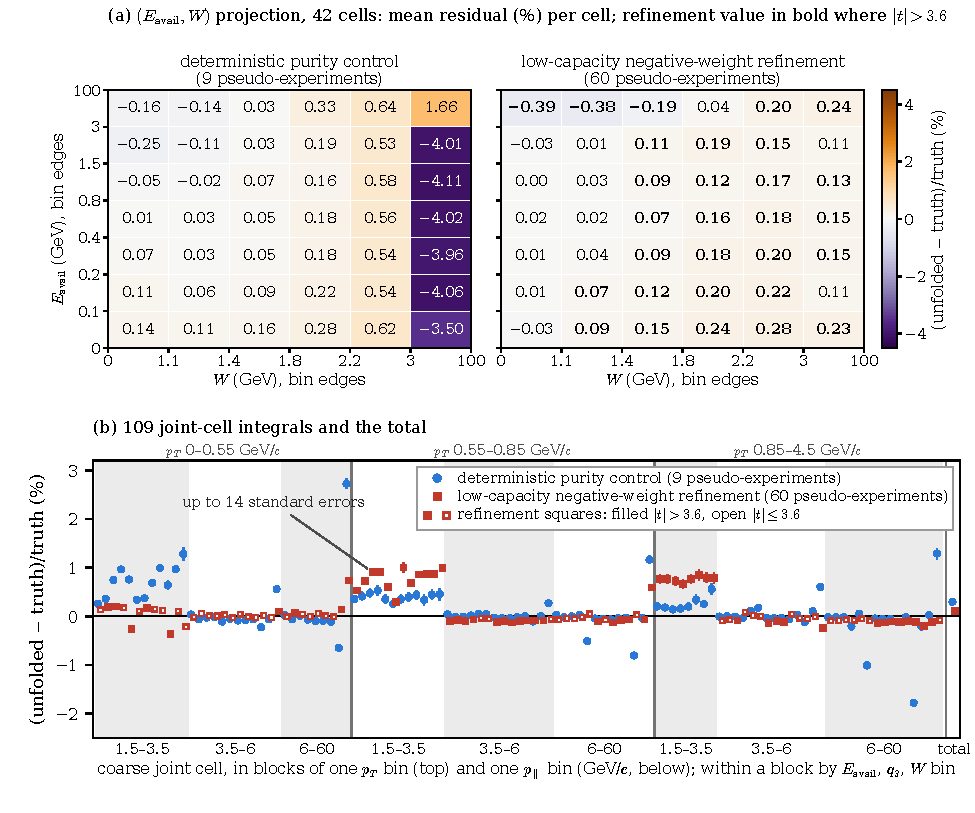
\includegraphics[width=\linewidth]{figures/paper_fig_bkg_residual.pdf}
  \caption{At nominal truth, the low-capacity negative-weight refinement reduces the closure residuals in the $(E_{\mathrm{avail}},W)$ plane, where the deterministic purity control is $3.5\%$ to $4.1\%$ low in most of the highest-$W$ column, but leaves residuals of about $1\%$ in some joint cells. Panel (a) maps the mean fractional closure residual with simulated backgrounds in the 42 $(E_{\mathrm{avail}},W)$ cells, for the deterministic purity control (9 pseudo-experiments, left) and the low-capacity negative-weight refinement (60 pseudo-experiments, right), on one colour scale. Panel (b) shows the same residuals for the \jtNcells{} supported joint cells, in blocks of one $p_T$ bin and one $p_\parallel$ bin, followed by the integrated total. There, circles show the purity control and squares the refinement, with error bars giving standard errors of the mean. The two ensembles are unpaired. The plot uses $t$ for the mean residual in standard errors. A refinement value is printed in bold, or its square filled, when $|t|>3.6$, the per-quantity threshold of the nominal closure criterion.}
  \label{fig:bkg-residual-note}
\end{figure}

The purity bias disappears in signal-only tests. In the widest mass bin, $W\geq3~\mathrm{GeV}$, the background yield is about $13\%$ of signal. Purity subtraction corrects the reconstructed bin integral, while the unbinned learner resolves background variation within the bin (Appendix~\ref{app:negative-weight-background}). On data, switching the subtraction method shifts the tested integrals by a median of $0.36\%$ and at most $1.4\%$.

\label{sec:val-departure}
The low-capacity refinement fails its recovery criterion for a generator-sized truth change. This stress test uses a GiBUU-to-GENIE $E_{\mathrm{avail}}$ shape ratio with weights from 0.70 to 1.33 at fixed total rate. The GENIE sample for this ratio used a mismatched flux. Appendices~\ref{app:bias-prior-stability} and~\ref{app:choices-after-results} document the mismatch and the decision to retain the original ratio. The median absolute residual in the $(E_{\mathrm{avail}},W)$ plane is $9.7\%$ and reaches $74\%$ in the highest-$W$ column. A separate change in the conditional $q_3$ distribution, with the $(E_{\mathrm{avail}},W)$ truth held fixed, shifts the unfolded cells in that plane by up to $37\%$. Both effects persist in signal-only repeats.

The sixteen-cell estimator recovers a median of $\fvval{rec-g-fmed}\%$ of the injected GiBUU-like change across supported cells of the $(E_{\mathrm{avail}},W)$ plane with injected changes larger than $2\%$ in magnitude. For three other generator-derived shapes, the median recovered fractions range from $\fvval{rec-w-fmed-lo}\%$ to $\fvval{rec-w-fmed-hi}\%$, with individual cells overshooting or moving opposite to the injected change (Appendices~\ref{app:bias-prior-stability}, \ref{app:reproducibility-definitions}, and \ref{app:choices-after-results}). In noise-free pseudo-data, raising the iteration count from five to thirty reduces the $E_{\mathrm{avail}}$ residual by $26\%$ while increasing the $q_3$ residual, and the quoted uncertainties of the \resFiveAxis{} do not include these residuals.

\subsection{Prior dependence and algorithmic robustness}
\label{sec:higher-dimensional-prior}
\label{sec:fived16-fd}

The sixteen-cell result depends on the starting distribution and on the unfolding procedure. The sixteen-cell estimator exceeds the prespecified bias criteria at \fvval{f0b-nlisted} of the \fvval{f0b-all-truths} simulated truths: the GiBUU hybrid, which uses GiBUU bin integrals and the MINERvA simulation within each fine bin, and a synthetic momentum-transfer tilt at fixed $(E_{\mathrm{avail}},W)$. The test compares the mean unfolded vector with the known truth using $C_{\mathrm{rep}}$. For truths derived from a generator in $C_{\mathrm{model}}$, it removes that generator's contribution. A truth is flagged if $p<\fvval{trig-p}$ or any cell has an absolute standardized residual $|z|>\fvval{trig-z}$ (\hyperlink{validation-sixteen-bias}{fake-data bias row} of Table~\ref{tab:validation-inventory}).

The GiBUU hybrid gives $\chi^2=\fvval{f0b-A7_gibuu-chi2}$ and $p=\fvval{f0b-A7_gibuu-p}$, with absolute standardized residuals $|z|>\fvval{trig-z}$ in the two low-$p_T$ cells with high available energy, low momentum transfer, and low mass (R02 and R06, Table~\ref{tab:five-dimensional-regions}). The synthetic $q_3$ tilt at fixed $(E_{\mathrm{avail}},W)$ gives $\chi^2=\fvval{f0b-q3-chi2}$ and $p=\fvval{f0b-q3-p}$, with $|z|\leq\fvval{trig-z}$ in every cell. Omitting the run-period term also flags the separate GiBUU $E_{\mathrm{avail}}$ shape through R06 at the same residual. Separate Poisson and noise-free checks at two held-out GENIE v3 tunes flag neither tune, and the largest cell bias is below \fvval{f1-bsig-ceil} of its reported standard deviation.

\label{sec:fived16-prr}
The sixteen-cell estimator recovers only part of the shift from the prior toward truth at both flagged truths. The signed fraction $\rho$ of the shift still missing along the prior-to-truth direction is
\begin{equation}
  \rho=-\frac{\sum_i b_i d_i}{\sum_i d_i^2},
  \qquad |d_i|\geq 0.01 ,
  \label{eq:five-dimensional-retained-prior}
\end{equation}
where $d_i=(X_i-P_i)/P_i$ and $b_i=(\widehat X_i-X_i)/P_i$ for prior, true, and unfolded integrals $P_i$, $X_i$, and $\widehat X_i$. This gives $\rho=0$ for exact recovery, $\rho=1$ for staying at the prior, and $\rho<0$ for overshooting along that direction. On noise-free samples with background, $\rho=\fvval{prr-rho-e-gibuu}$ at the GiBUU hybrid and $\fvval{prr-rho-e-q3}$ at the $q_3$ tilt. Reducing classifier capacity or using only muon momenta increases retention at both truths. Dropping $W$ alone or dropping both $W$ and $q_3$ changes $\rho$ by less than \fvval{prr-s53-w-dmax}. None of the tested changes in iterations, capacity, training statistics, or inputs reduces retention by \fvval{prr-floor} or removes either bias flag. A second prespecified study on the same noise-free samples found that the retention at the GiBUU hybrid is consistent with a limit set by the weights of missed events. At the $q_3$ tilt, it is consistent with a limit set by the representation in the second, truth-level step. Both results match the pseudo-data at reconstruction level despite the residual at truth level, consistent with directions that the reconstructed inputs constrain weakly. Appendix~\ref{app:bias-prior-stability} gives the substitution tests, including the checks with true weights available only in simulation.

Five-iteration binned IBU overshoots along the prior-to-truth direction, with $\rho=\fvval{prr-rho-ibu-gibuu}$ and $\fvval{prr-rho-ibu-q3}$ for the two truths. It clears the flag for the $q_3$ tilt, retains the flag at the GiBUU hybrid, and flags \fvval{prr-ibu5-nnew-word} other truths. The two procedures discretize the problem differently, so the comparison also includes the effect of the chosen response grid.

\label{sec:fived16-ibu}
On data, binned IBU and the sixteen-cell estimator differ beyond the prespecified agreement thresholds, and the reported uncertainties do not include this difference. Both use \lrval{rg1-K} iterations, the same data, simulation, background template, and weight-only systematic universes, and their outputs are integrated over the same sixteen regions. For the difference $\Delta$ we obtain $\Delta^{\mathsf T}C_\Delta^{-1}\Delta=\lrval{rg1-T}$, compared with calibrated \fpeval{100*\lrval{rg1-lev1}}th and \fpeval{100*\lrval{rg1-lev2}}th null percentiles of \lrval{rg1-bar1} and \lrval{rg1-bar2}. The covariance $C_\Delta$ propagates statistical, weight-only systematic, and normalization variations through both estimates, but not the model, lateral, response, or run-period terms.

\label{sec:3d-classifier}
A descriptive comparison of tree and multilayer-perceptron classifiers finds similar 3D purity projections in the tested configuration (Appendix~\ref{app:algorithm-classifier-controls}).

\label{sec:gbdt-model-dependence}
Coarsening the reporting grid leaves substantial dependence on the starting model. In a precision study with generator-sized departures, all three grids miss the $5\%$ model-component and $75\%$ recovery targets, including the \fvval{h2-nsupported} supported joint boxes used to define the sixteen cells (Appendix~\ref{app:bias-prior-stability}). On the sixteen cells, $C_{\mathrm{model}}$ summarizes shifts on data when the prior is reweighted toward GENIE with meson-exchange currents, NuWro, or GiBUU. These shifts measure sensitivity to the chosen priors and carry no calibrated bound on the bias.

\subsection{Numerical stability and covariance limits}
\label{sec:higher-dimensional-calibration}
\label{sec:5d}

The sixteen-cell estimator fails the prespecified rounding-stability test on data, with shifts of 0.8 at the median and up to \lrval{stab-max} statistical standard deviations, against tolerances of \fvval{ens1-bar-median} and \fvval{ens1-bar-max} (\hyperlink{validation-sixteen-rounding}{rounding-level stability row}). The shifts are measured over the joint-cell integrals, the $E_{\mathrm{avail}}$--$W$ integrals and their sum, and the total rate. The test perturbs each stored input by up to half a single-precision unit in the last place and holds fine-grid bin membership fixed. Appendix~\ref{app:bias-prior-stability} compares the low-capacity, averaged, cross-fitted, and regularized variants under the same test, including the stricter pseudo-data comparison.

\label{sec:eavailw-adopted}
The fine-grid purity covariance $C_Z$ serves as a descriptive scale only. It did not meet the requirements for inference. Two companion builds exceeded the $\sprojBound\%$ training-seed tolerance, with a largest shift of $\sprojMeasured\%$ in a projected standard deviation. The criterion was uncomputed for $C_Z$ itself. The comparison held the seed fixed for five systematic bands that carry $\pinnedBandsSqrtTr\%$ of $\sqrt{\operatorname{Tr}C_Z}$ (Appendix~\ref{app:multidimensional-statistics}).
% Search: s_proj; M(ii); cause 3; C3; estimator-seed magnitude criterion; z-cv 3d7465f6; GRADE-20260920; VL146; L2 (computed only for 361090f9/7e4636a3, DECISION-20260920-joseph-adopts-z-cv-under-the-6.4-exception.md:36-38; z-cv precursor undeclared so branch 3 unreachable, EVIDENCE-20260919-cause3-member-eligibility-census.md:17-19; later s_proj on other products only, VALIDATION_LEDGER.md:219, OUTCOME-20260922-L2-sproj-measured-and-the-pair-is-not-code-comparable.md:3-5) @ 0d919b1a

Separately, data from different run periods are inconsistent before unfolding, and the run-period term was constructed after the differences were observed (Sec.~\ref{sec:sixteen-cell-projections}).

Table~\ref{tab:higher-dimensional-validation} summarizes the tests by estimator.

\begin{table}[tbp]
  \centering
  \linespread{1}\footnotesize
  \caption{Principal higher-dimensional validation tests. A criterion is prespecified if it was recorded before its outcome was read. Appendix~\ref{app:validation-inventory} gives the complete inventory.}
  \label{tab:higher-dimensional-validation}
  \begin{tabular}{@{}>{\raggedright\arraybackslash}p{0.213\textwidth}
                      >{\raggedright\arraybackslash}p{0.21\textwidth}
                      >{\raggedright\arraybackslash}p{0.25\textwidth}
                      >{\raggedright\arraybackslash}p{0.25\textwidth}@{}}
    \toprule
    Test & Estimator or result & Outcome & Consequence \\
    \midrule
    $E_{\mathrm{avail}}$ and $q_3$ bumps (descriptive) &
    3D and 4D purity baseline &
    Marginal residuals $1.84\%$ and at most $1.1\%$. &
    Recovery characterized for two smooth marginal features. \\
    \addlinespace[2pt]
    $W$ bump (prespecified) &
    5D purity baseline, signal only &
    Marginal ratio 0.180 passes the 0.20 limit. &
    Joint peak-column cells remain up to $9.4\%$ low. \\
    \addlinespace[2pt]
    Nominal truth with backgrounds (descriptive) &
    Deterministic purity control, low-capacity refinement, and sixteen-cell estimator &
    Negative-weight treatment reduces the high-$W$ bias. &
    Improvement established at nominal truth for the tested treatments. \\
    \addlinespace[2pt]
    Generator-sized recovery (prespecified) &
    Low-capacity refinement control &
    Fails with a median $9.7\%$ residual on the $(E_{\mathrm{avail}},W)$ plane. &
    Large joint residuals persist with signal only. \\
    \addlinespace[2pt]
    Reporting-resolution precision (prespecified) &
    Sixteen-cell estimator and its admissible settings on three diagnostic grids &
    Prior sensitivity exceeds the $5\%$ target on all three. &
    Coarsening leaves appreciable model dependence. \\
    \addlinespace[2pt]
    Fake-data bias (prespecified) &
    Sixteen-cell estimator &
    GiBUU hybrid and $q_3$ tilt exceed the criteria. &
    Bias exceeds the allowed scale under the reported covariance. \\
    \addlinespace[2pt]
    Classifier-family comparison (descriptive) &
    3D purity baseline &
    Median projection differences $0.7\%$--$1.4\%$. &
    Agreement applies to the tested 3D projections. \\
    \addlinespace[2pt]
    Binned IBU comparison (prespecified) &
    Sixteen-cell estimator and binned IBU &
    Difference exceeds the calibrated thresholds. &
    Joint cell estimates depend on the unfolding procedure. \\
    \addlinespace[2pt]
    End-to-end coverage (prespecified) &
    Deterministic purity control, statistical intervals &
    Fails the futility rule at nominal and reduced rates. &
    Coverage fails for this estimator variant. \\
    \addlinespace[2pt]
    Held-out-tune coverage (descriptive) &
    Sixteen-cell estimator with $C_{\mathrm{total}}$ &
    Joint undercoverage at both tunes. &
    Also too small with the full reported covariance. \\
    \addlinespace[2pt]
    Rounding-level stability (prespecified) &
    Sixteen-cell estimator &
    Fails with shifts up to $\lrval{stab-max}$ statistical standard deviations. &
    Central values are sensitive to rounding-level changes. \\
    \addlinespace[2pt]
    Covariance seed tolerance (prespecified) &
    Companion purity covariance builds &
    Projected shifts exceed the $\sprojBound\%$ tolerance. &
    Part of the seed sensitivity remains unmeasured. \\
% Search: s_proj; M(ii); cause 3; estimator-seed magnitude criterion; GRADE-20260920; VL146; L2 (the search of this section's seed paragraph at 0d919b1a, rerun; no OUTCOME, DECISION, GRADE or EVIDENCE record changes an s_proj mention since 0d919b1a) @ caae27166e85
    \addlinespace[2pt]
    Muon-quadrant sums (prespecified) &
    Sixteen-cell and 2D results &
    Passes the comparison rule. &
    Supports consistency of the coarse muon projection. \\
    \bottomrule
  \end{tabular}
\end{table}

\subsubsection{Closure at held-out tunes and interval diagnostics}
\label{sec:closure-interval-diagnostics}

Closure tests compare unfolded pseudo-data with known truth. The mean residual measures method bias at that truth, and the fraction of intervals or joint regions containing the truth measures coverage. Neither reported covariance includes a term estimated from closure at held-out tunes. The sixteen-cell covariance includes the prior-shape term, and the 2D result reports it separately as $C_{\mathrm{model}}$. Any residual bias would need to be accounted for as a systematic uncertainty before the results could be used to constrain models.

\phantomsection\label{sec:coverage-tunes} The 2D joint regions contain the truth in \lrval{cov2d-ar23-joint} of \lrval{cov2d-ntoys} pseudo-experiments at \fvval{f1-tune-ar23} and \lrval{cov2d-g18-joint} of \lrval{cov2d-ntoys} at \fvval{f1-tune-g18}, the two held-out GENIE v3 tunes. These tests use covariances rebuilt at each tune with the prior-shape term and with the run-period block omitted. The mean $\chi^2/\mathrm{ndf}$ is $\lrval{cov2d-ar23-chi2ndf}\pm\lrval{cov2d-ar23-chi2ndf-se}$ and $\lrval{cov2d-g18-chi2ndf}\pm\lrval{cov2d-g18-chi2ndf-se}$, respectively. Rescoring with the run-period block gives \fvval{rg-2d-ar23-full} and \fvval{rg-2d-g18-full}, still far above the expected value of about 1.

\begin{samepage}
\phantomsection\label{sec:sixteen-cell-closure-tunes} For the sixteen-cell cross section, the joint regions contain the truth in \fvval{ll5d-njoint-min} to \fvval{ll5d-njoint-max} of \fvval{ll5d-ntoys} draws across both tunes and band variants. The counts use the covariance subtotal $C_{\mathrm{total}}$ before the response and run-period terms. Part of the procedure was fixed after an early stop. The scoring criteria were prespecified, and the counts are descriptive. They do not constitute a calibrated coverage test (Appendix~\ref{app:choices-after-results}).\par
\end{samepage}

Rescoring with the reported covariance $C_{\mathrm{rep}}$ lowers the mean $\chi^2/\mathrm{ndf}$ from \fvval{rg-16-orig-min}--\fvval{rg-16-orig-max} to \fvval{rg-16-full-min}--\fvval{rg-16-full-max}. The reported covariance is still too small for these residuals. An end-to-end test would also need to draw the response and run-period variations, which were absent from these draws. Appendix~\ref{app:closure-interval-diagnostics} gives the joint-containment equation and thresholds, the per-bin results, the earlier statistical-band test, the pull diagnostic, and the 5D purity-control coverage test and figure.

% PASS2: The supplied source prints the other numerical literals as literals (including literal arguments to \SI and \SIrange). The unmatched draft-specific values are 6.74e-41 (the spectrum figure annotation; sec_3d.tex prints 6.7e-41), the Eavail--W map readings (1.23--1.26, 1.30, and 4.1e-40, plus their bin limits), and the full muon-axis ranges [0,4.5] and [1.5,60] (only the three-edge lists and individual boxes are macroized). The 1000 support threshold is literal in the multidimensional statistical methods. R02 and R06 are cell identifiers. The 26.0% trace claim is unchanged. sec_5d.tex prints \pinnedBandsSqrtTr (26.0%) for the square root of the trace, while \pinnedBandsTrace is 6.75%. The precision-study row retains its wording. sec_5d.tex identifies the sixteen-cell estimator as the raised-capacity estimator used for repeated experiments, while its reporting-resolution selection considered multiple admissible configurations. Confirm the intended scope of that row. All references in this section have local or manuscript targets. The legacy labels tab:test-index and tab:closure-map belong on the full inventory in App. A.6 (tab:validation-inventory). sec:fived16 and sec:fived16-result belong to Sec. 5.1. The C_Z construction anchors sec:eavailw-construction, eq:zassembly, and eq:zinflation belong in App. A.4. The legacy tab:fived16-cells points to the retained geometry table here. The cross-section table is in Sec. 5.1. The five graphics paths match the manifest. The real PDFs were not supplied in this workspace. The two-panel placement of paper_fig2_joint was tested with a stand-in from the supplied note and should be checked on the real PDF.
